% Drawing 74/07-3 -- folder 74, batch 07, archive page 125 (PDF page 126).
% Transcription: un graphe aux sommets $s'$, $s$, $u'$, $u$, $t$, $a$, $b$, $c$, $y'$.
% Kind: graph (pentagon with star). Method 2 (schematic redraw from the facsimile). Status: partial.
% Notes: A pentagon-shaped graph with apex s': the outline s' - s - u - c - b and s' to the right edge (t); inside, s' - a, s - a, a - b, a - c, u' - c, and two near-horizontal strokes from u and u' to the right; every edge between the same vertex points. Letters small and placed by reading (s', s, u', u, t, a, c as in the transcription; b at the lower right corner by guess, y' not found in the crop). A small triangle sketch at the bottom of the page with the letters s s', a, b, c, t t', y y', u a', z z' has no mark of its own and may be what the transcription lists. Still differs: the right part is cut by the bbox edge, where t stands; which inner strokes end at a is partly a reading. Nothing is struck. Redrawn 2026-11-09 (issue 128): to check again.
% Coordinates: 1 unit = 1 mm = 1/100 of the crop width (bbox in page fractions: [0.6, 0.15, 0.85, 0.35]).
% Redrawn by Claude (claude-opus-5-5), issue #73, 2026-11-09; not checked by a human; not compiled (no TeX in the session).
% Rights: reproduces part of the work -- behind RENDER_TRANSCRIPTS, never published by itself.
\documentclass[tikz,border=3pt]{standalone}
\usepackage{amsmath,amssymb}
\usetikzlibrary{patterns,arrows.meta}
\tikzset{pencil/.style={black!45}, struck/.style={black!35}, mark/.style={circle,draw,inner sep=1.3pt}, pt/.style={circle,fill,inner sep=0.9pt}, opt/.style={circle,draw,fill=white,inner sep=1.1pt}}
\begin{document}
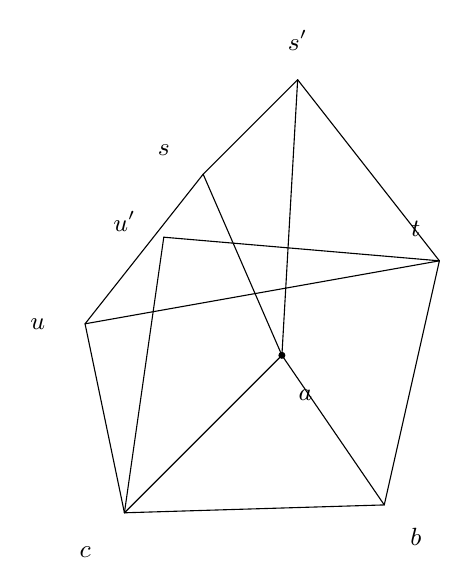
\begin{tikzpicture}[x=1mm,y=1mm,line cap=round,line join=round,font=\scriptsize]
\draw (82,-48) -- (70,-60);
\draw (70,-60) -- (55,-79);
\draw (55,-79) -- (60,-103);
\draw (60,-103) -- (93,-102);
\draw (93,-102) -- (100,-71);
\draw (100,-71) -- (82,-48);
\draw (82,-48) -- (80,-83);
\draw (70,-60) -- (80,-83);
\draw (80,-83) -- (93,-102);
\draw (80,-83) -- (60,-103);
\draw (65,-68) -- (60,-103);
\draw (55,-79) -- (100,-71);
\draw (65,-68) -- (100,-71);
\node[pt] at (80,-83) {};
\node[inner sep=1pt] at (82,-43) {\small $s'$};
\node[inner sep=1pt] at (65,-57) {\small $s$};
\node[inner sep=1pt] at (60,-66) {\small $u'$};
\node[inner sep=1pt] at (49,-79) {\small $u$};
\node[inner sep=1pt] at (55,-108) {\small $c$};
\node[inner sep=1pt] at (97,-106) {\small $b$};
\node[inner sep=1pt] at (97,-67) {\small $t$};
\node[inner sep=1pt] at (83,-88) {\small $a$};
\end{tikzpicture}
\end{document}
